% Created 2024-10-03 Thu 23:07
% Intended LaTeX compiler: pdflatex
\documentclass[12pt]{article}
\usepackage[utf8]{inputenc}
\usepackage[T1]{fontenc}
\usepackage{graphicx}
\usepackage{longtable}
\usepackage{wrapfig}
\usepackage{rotating}
\usepackage[normalem]{ulem}
\usepackage{amsmath}
\usepackage{amssymb}
\usepackage{capt-of}
\usepackage{hyperref}
\usepackage[margin=1in]{geometry} \usepackage{amsmath}
\author{Jason Press}
\date{\today}
\title{Breaking Fishing Line}
\hypersetup{
 pdfauthor={Jason Press},
 pdftitle={Breaking Fishing Line},
 pdfkeywords={},
 pdfsubject={},
 pdfcreator={Emacs 29.4 (Org mode 9.7.11)}, 
 pdflang={English}}
\begin{document}

\maketitle
\section{Introduction}
\label{sec:org6c10fd9}

In this lab, we added an increasing amount of mass to a mass hanger suspended by two fishing lines, one rated for four pounds of force and the other rated for eight pounds of force. The goal of the lab was to predict which line would break first. To obtain the maximum amount of tension each line can handle, we added an increasing amount of mass to a mass hanger suspended by one line until the line broke. The amount of mass that the string held before it broke is the maximum amount of weight \(m\) it can hold, so the amount of tension the line can handle is \(mg\).

In the setup, let \(m_1\) be the line of choice, \(\theta_1\) the angle that line \(m_1\) makes from the mounting point, \(M_1\) the maximum amount of tension that \(m_1\) can handle, and \(\theta\)\textsubscript{2} the angle that the other line makes from the mounting point. For a visual depiction, see Figure \ref{fig:setup}. This equation gives the maximum amount of weight \(m_1\) can handle before snapping in the experimental setup:

\begin{align}\label{eq:tension}
m_{weight,1} = M_{1} \left( \sin\theta_1 + \cos\theta_1\tan\theta_2 \right)
\end{align}

The amount of weight \(m_2\) can handle also uses Equation \ref{eq:tension}, with \((1,2 := 2,1)\). The maximum amount of weight that the experimental setup can handle is therefore \(\min(m_{weight,1}, m_{weight,2})\).
\section{Methods}
\label{sec:org8e53272}

This lab has two components: the experimental setup, with the hanging mass suspended by two fishing lines; and testing each line for tension.
\subsection{The Experimental Setup}
\label{sec:org94cd7a6}

For the experimental setup, we tied both lines to the ceiling on two convenient locations, some arbitrary distance apart. Then, we tied each line to the mass hanger, labeled \texttt{w} in Figure \ref{fig:setup}. After predicting the result, we tested the prediction by placing more and more mass on the mass hanger until one line snapped, causing the whole setup to fall to the ground (the second line snapped after the first due to the lack of support from the first line).

\begin{center}
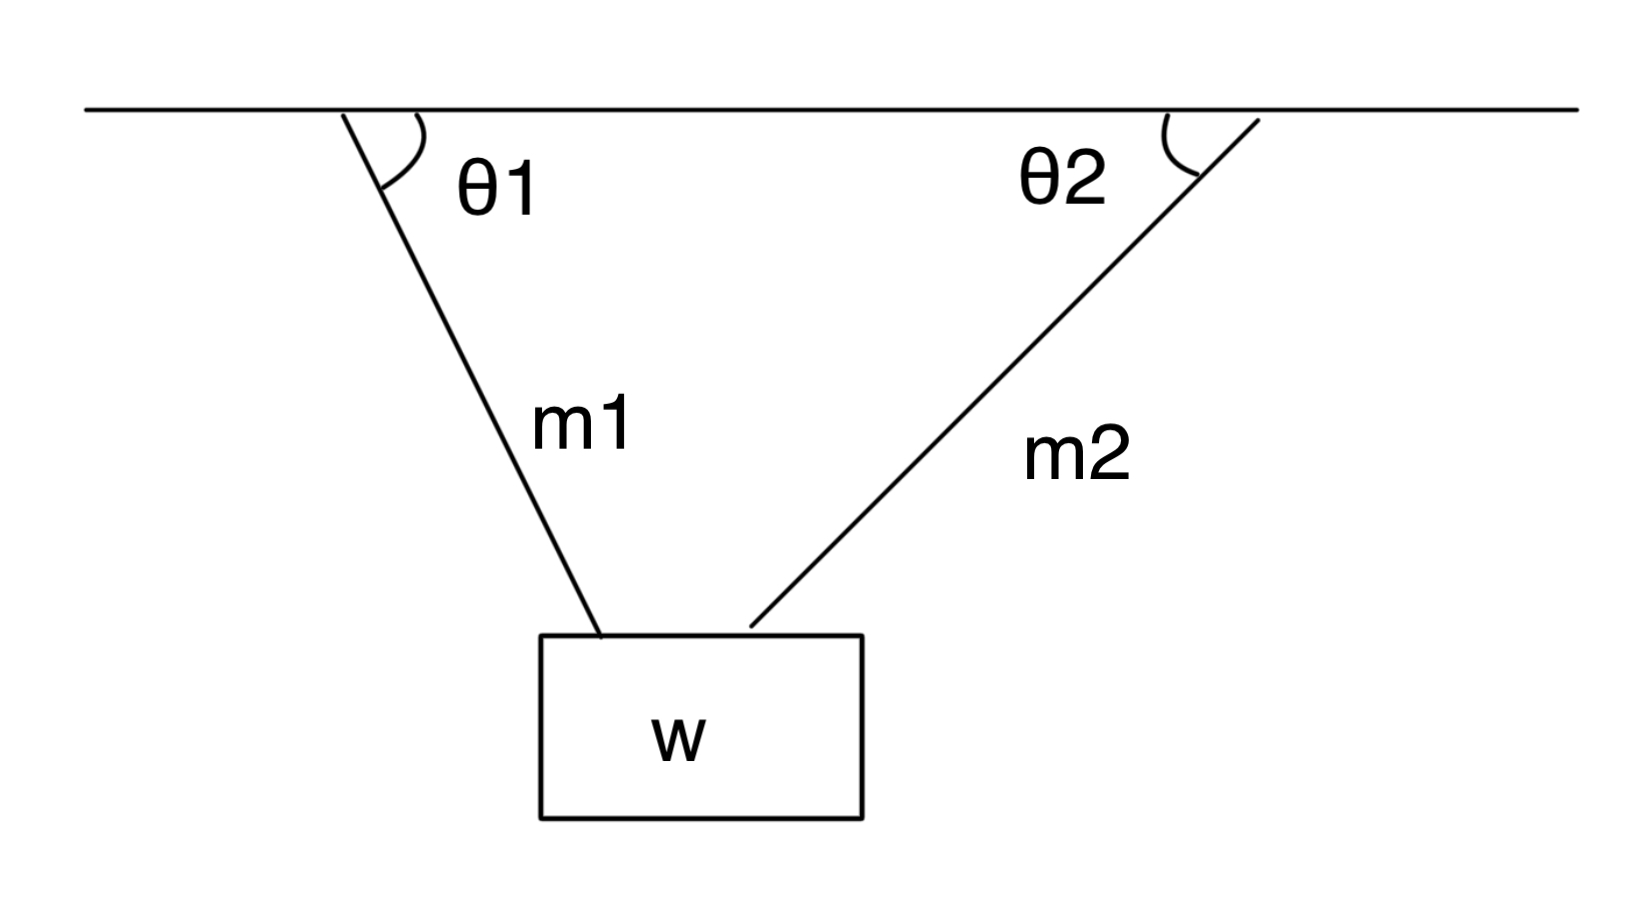
\includegraphics[width=6.5in]{./lab4diagram.png}
\captionof{figure}{\label{fig:setup}Experimental setup}
\end{center}
\subsection{The Testing Setup}
\label{sec:org6e44a0f}

For the testing setup, we tied one piece of line to a convenient location, a cross beam in the lab, and the other to a mass hanger.

\begin{center}
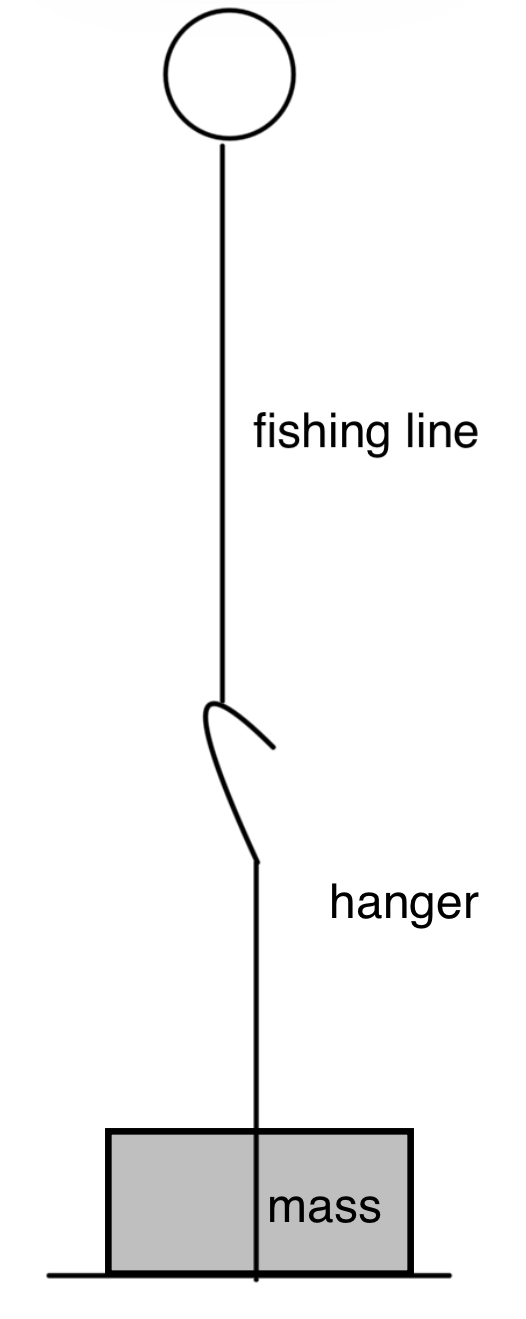
\includegraphics[height=5in]{./lab4hanger.png}
\captionof{figure}{\label{fig:test}Testing a line for its carrying capacity}
\end{center}
\section{Results}
\label{sec:org3ee95c9}

\section{Discussion}
\label{sec:orgf65ec6d}

\section{Sample Calculations}
\label{sec:org280700f}
\end{document}
